\section{Архитектура системы}

Для реализации требований была разработана распределённая микросервисная архитектура,
которая состоит из нескольких основных и инфраструктурных компонентов и представлена на рисунке \ref{architecture}.

\begin{figure}[ht]
\begin{center}
\scalebox{0.25}{
   
\includegraphics{images/architecture.png}
}
\caption{
\label{architecture}
     Архитектура системы.}
\end{center}
\end{figure}

\subsection{Интерфейс взаимодействия с пользователем}

Компонент представляет собой web-приложение, разработанное с использованием React JS.
Он обеспечивает взаимодействие пользователя с системой.

Использование web-приложения позволяет обеспечить кроссплатформенность системы, так как для работы требует наличие любого браузера.
Взаимодействие Frontend-приложения с Backend-компонентами осуществляется по HTTP и WebSocket через nginx.
Nginx используется в качестве обратного прокси и балансировщика нагрузки.

В качестве подхода к структурной схеме приложения был выбран Feature Sliced Design (FSD).
Он предполагает разделение кода на независимые и переиспользуемые модули и слои,
что упрощает сопровождение и развитие системы при появлении новых функциональных требований.
Структура веб-приложения представлена на рисунке \ref{frontend-structure}.

\begin{figure}[ht]
\begin{center}
\scalebox{0.2}{
   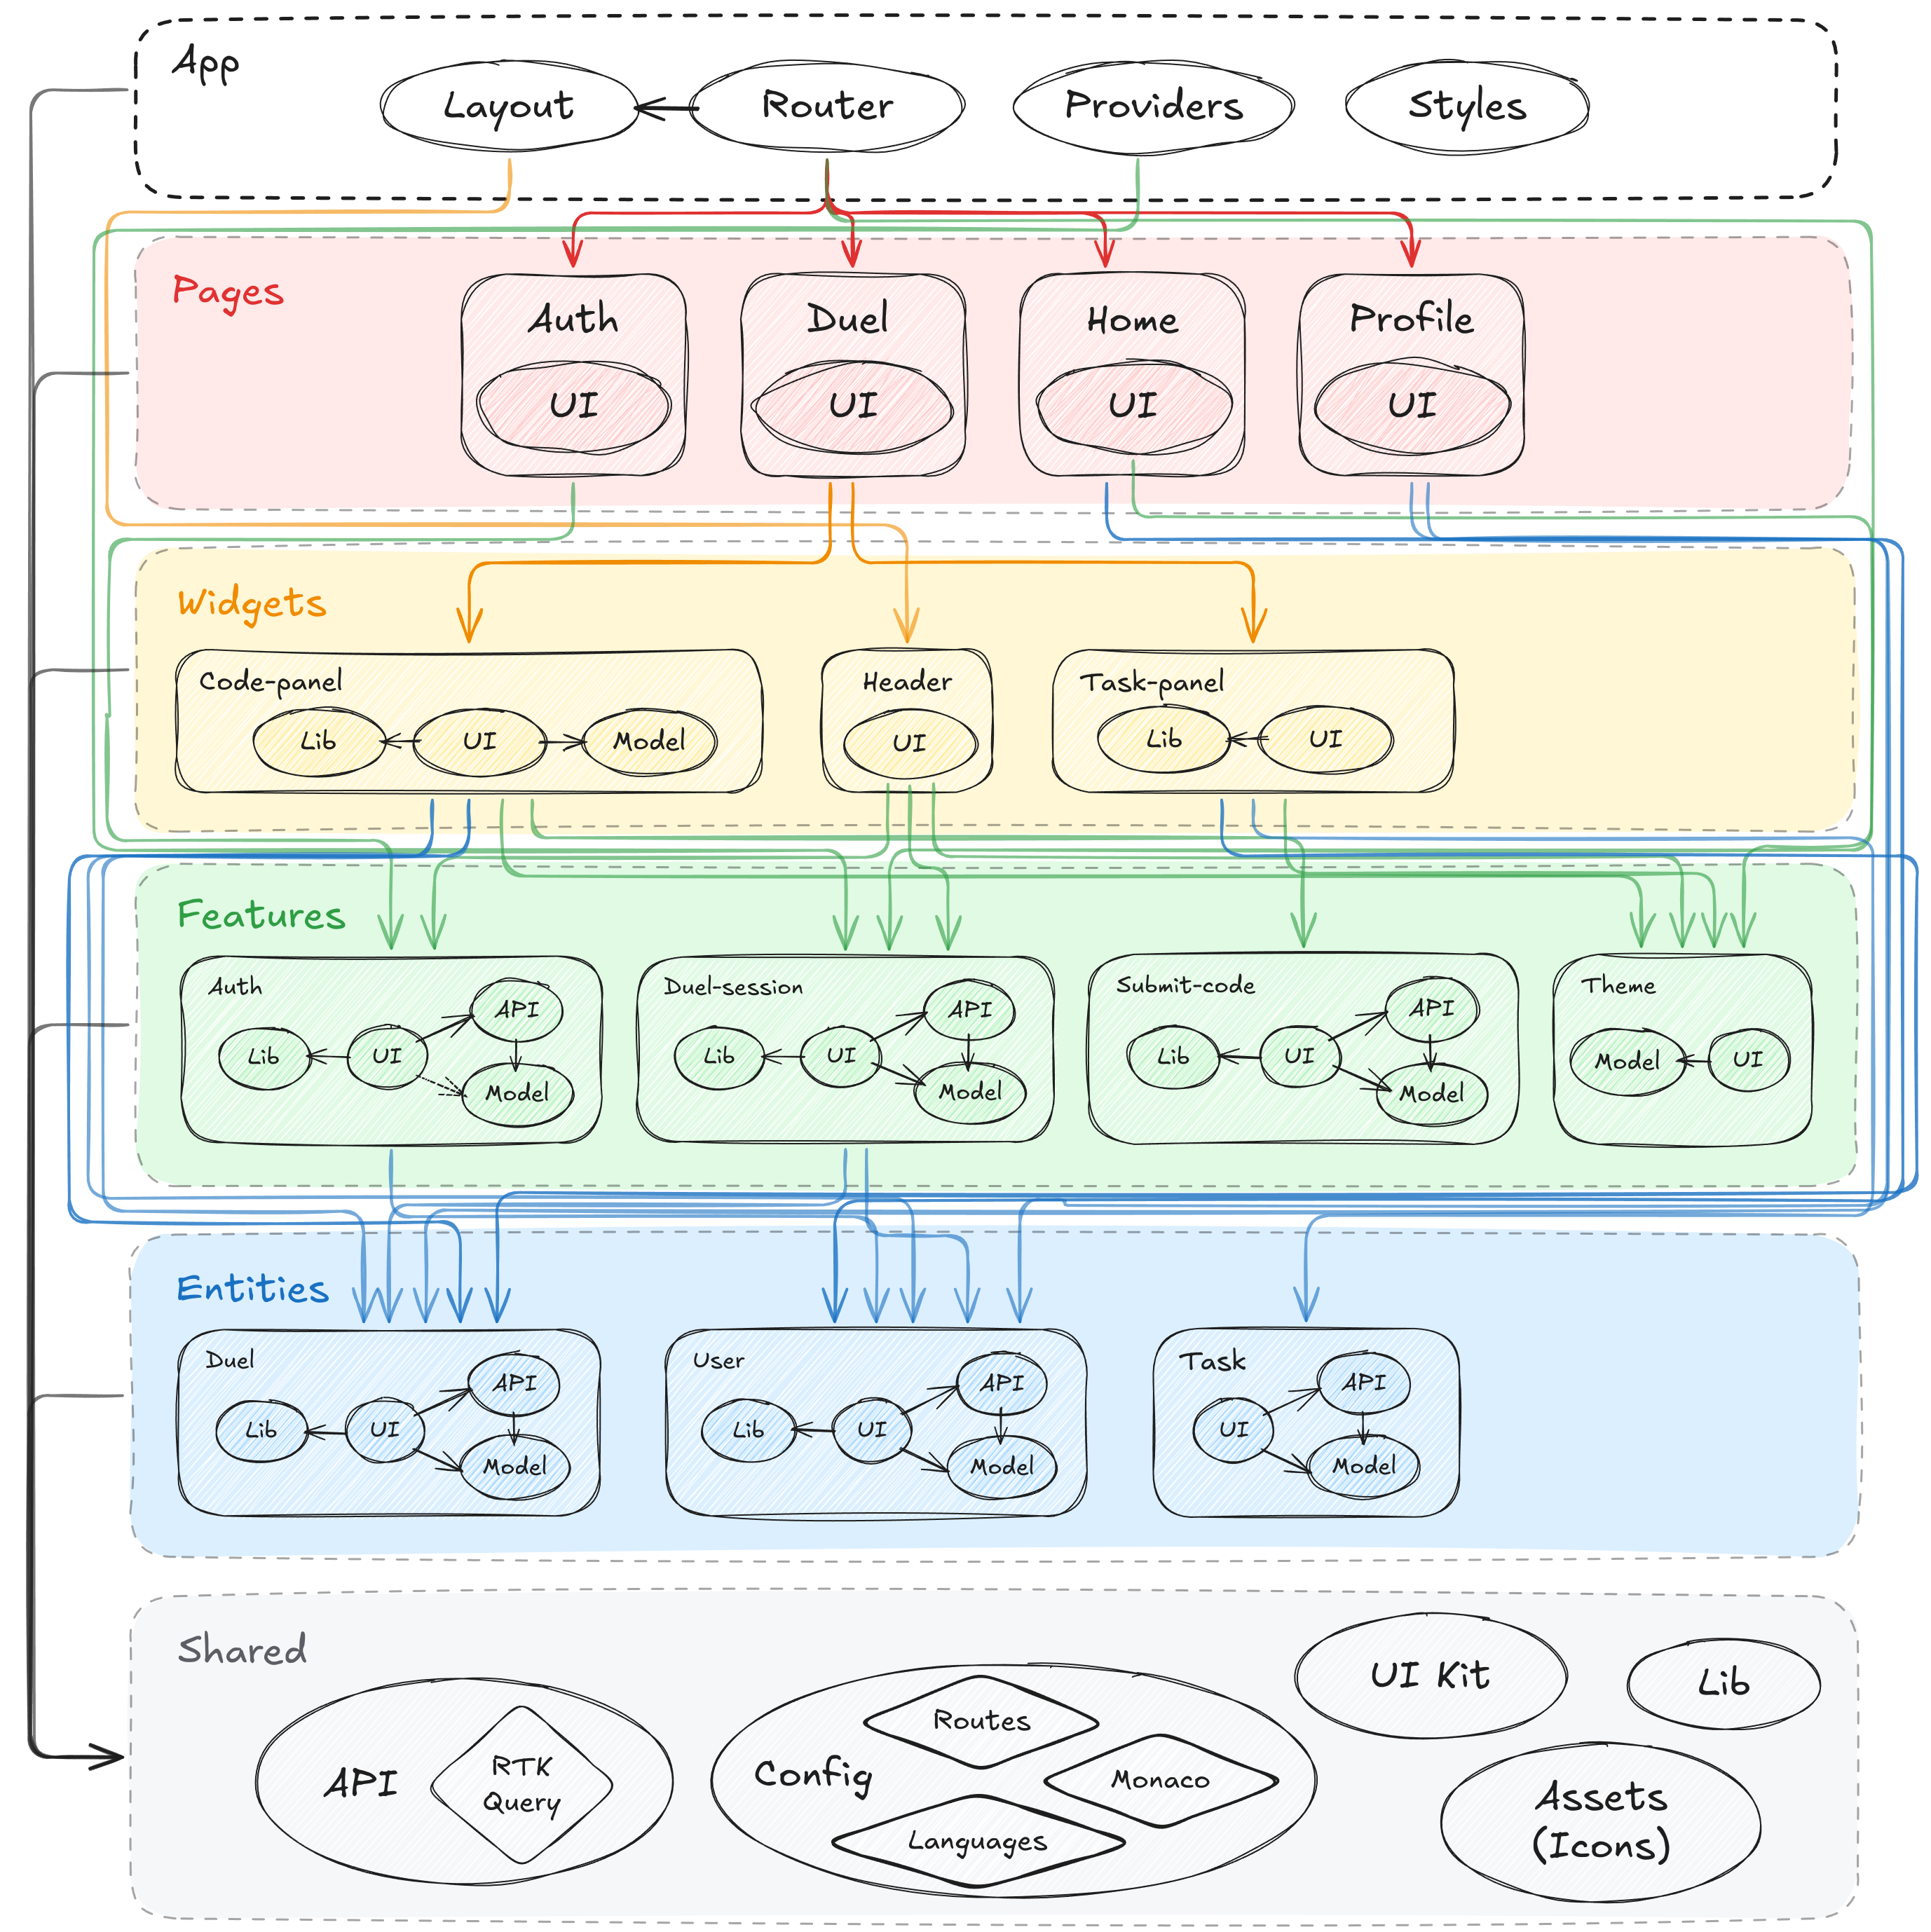
\includegraphics{images/frontend-structure.png}
}
\caption{
\label{frontend-structure}
     Структура веб-приложения.}
\end{center}
\end{figure}

В качестве редактора кода в web-интерфейсе используется библиотека Monaco Editor.
Редактор схож с VS Code и поддерживает подсветку синтаксиса, работу с несколькими языками программирования,
а также предоставляет возможность сбора списка действий пользователя во время написания кода.

Приложение поддерживает выбор светлой и тёмной темы интерфейса, что позволяет повысить удобство использования системы
при различных условиях освещения и длительной работы с платформой.

\subsection{Компонент управления пользователями и дуэлями}

Компонент Duely представляет собой приложение на C\# с использованием ASP.NET,
в котором реализуется логика взаимодействия с пользователями,
а также бизнес-логика, относящаяся к управлению группами, проведению дуэлей и турниров.
Кроме того компонент отвечает за приём решений пользователей и их передачу в подсистему автоматического тестирования.

Подход к структуре приложения сочетает в себе подходы из чистой и гексагональной архитектуры.
Код приложения разбит на .NET-проекты (модули) с целью фиксации направлений зависимостей компонентов друг от друга.
Структура приложения Duely представлена на рисунке \ref{duely-structure}.

\begin{figure}[ht]
\begin{center}
\scalebox{0.2}{
   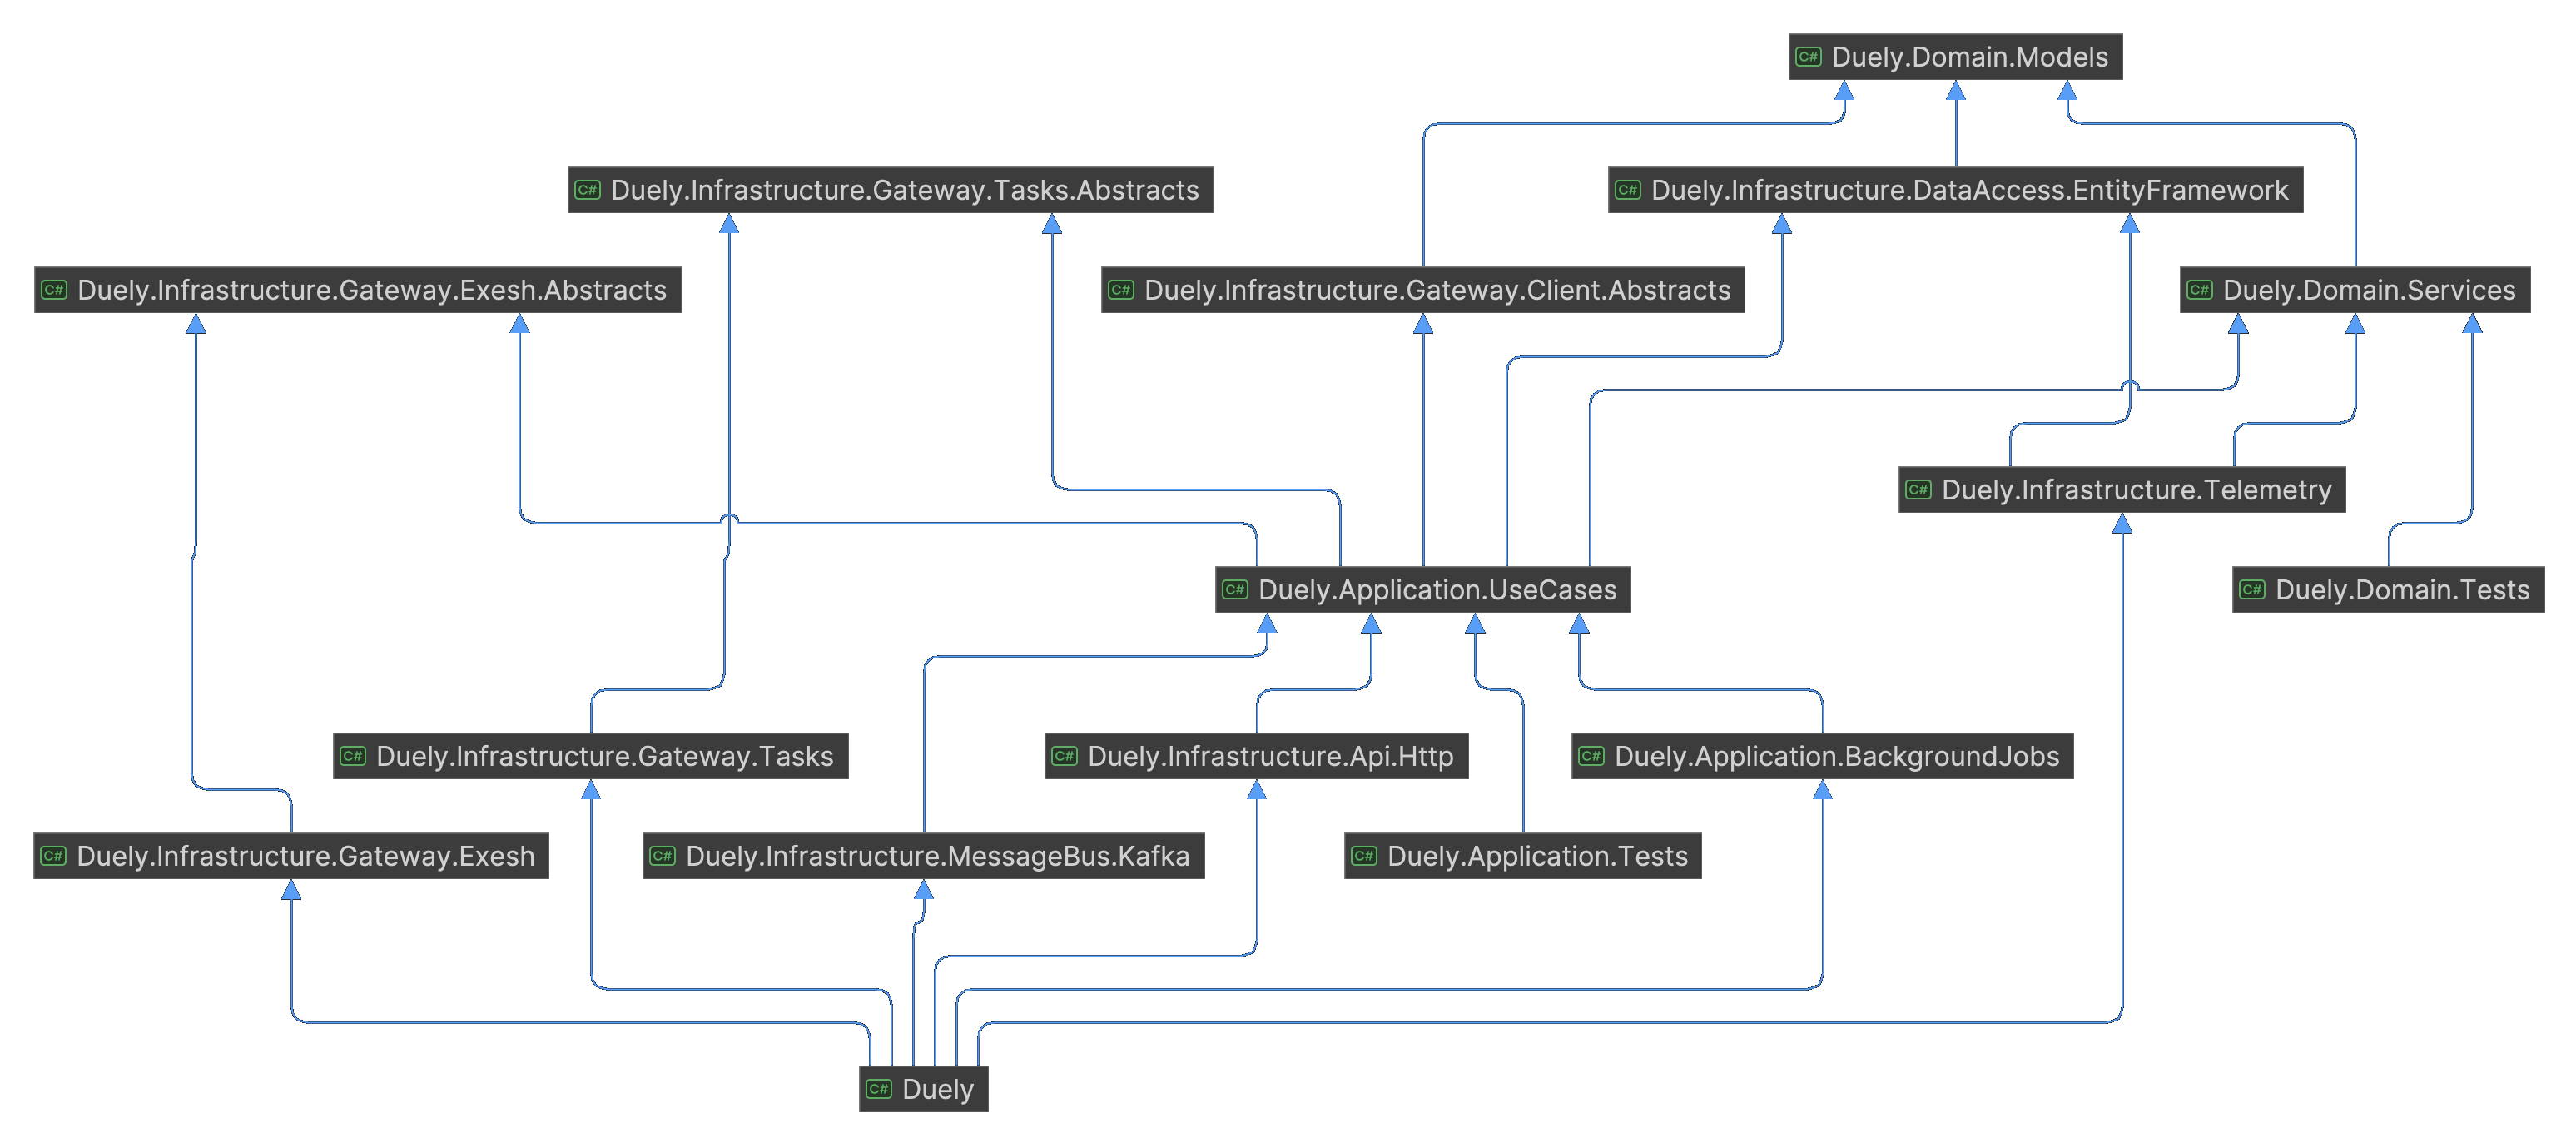
\includegraphics{images/duely-structure.png}
}
\caption{
\label{duely-structure}
     Структура приложения Duely.}
\end{center}
\end{figure}

В качестве базы данных используется PostgreSQL.
Выбор был сделан, исходя из широких возможностей СУБД для работы с реляционными данными,
поддержкой транзакционности и относительной простотой эксплуатации.
Для работы с БД в коде приложения и миграции схемы данных используется Entity~Framework.

Для авторизации запросов используется JWT токен, который выписывается при аутентификации по никнейму и паролю пользователя.
При выписке access токена также выписывается refresh токен, который используется для обновления access токена при окончании действия.

Используется двунаправленное WebSocket соединение с Frontend,
по которому отправляются события изменения кода пользователя в редакторе, а также изменения статуса тестирования решения.
Для авторизации запроса на установление соединения используется одноразовый token,
который выписывается компонентом Duely и прикладывается приложением Frontend к запросу на WebSocket соединение.

Для реализации взаимодействия с другими компонентами, вызванного реакцией на произошедшее в системе событие,
используется паттерн транзакционный Outbox.
Вместе с обновлением данных доменных моделей в БД сохраняется запись в таблицу Outbox о том,
о необходимости выполнения некоторого отложенного действия (например, отправить сообщение определённому пользователю в WebSocket).
Запущенный фоновый процесс сканирует записи этой таблицы, выполняет диспетчеризацию и необходимую обработку.
Использование данного паттерна позволяет добиться гарантии обработки события At~Least~Once.

\subsection{Компонент анализа поведения пользователя}

Компонент Analyzer представляет собой приложение на Python, предназначенное для анализа действий пользователя во время дуэли.

При помощи библиотеки FastAPI реализовано API,
с помощью которого можно получить степень подозрительности пользователя по списку его действий во время дуэли.
Для анализа степени подозрительности с использованием библиотеки scikit-learn реализованы и обучены ML-модели.

\subsection{Компонент менеджмента задач}

Компонент Taski представляет собой приложение на Go и используется для хранения и управления задачами,
а также определяет правила автоматического тестирования решений и вердикты тестирования.

Выделение управления задачами в отдельный компонент позволяет независимо от других компонентов развивать и использовать компонент.
Структура доменного слоя позволяет расширять систему новыми типами задач и сценариями их тестирования
без необходимости существенного изменения других компонентов системы.

В компоненте реализован свой формат хранения метаданных о задаче, а также конвертер из общепринятого формата polygon во внутренний.
Все файлы, необходимые для тестирования задачи (тесты, решение, чекер), хранятся в файловой системе.
Взаимодействие с файловой системой выполняется при помощи библиотеки filestorage.

\subsection{Компонент запуска команд тестирования}

Компонент Exesh представляет собой приложение на Go и используется для запуска произвольных команд, необходимых для тестирования задач.

Внутренняя архитектура Exesh представлена на рисунке \ref{exesh-architecture}
и включает два вида компонентов, которые образуют модель оркестрации.
Центральным компонентом является coordinator.
В нём содержится API, а также вся логика управления исполнением команд.
За выполнение команд и сохранение артефактов запуска отвечает worker.

\begin{figure}[ht]
\begin{center}
\scalebox{0.4}{
   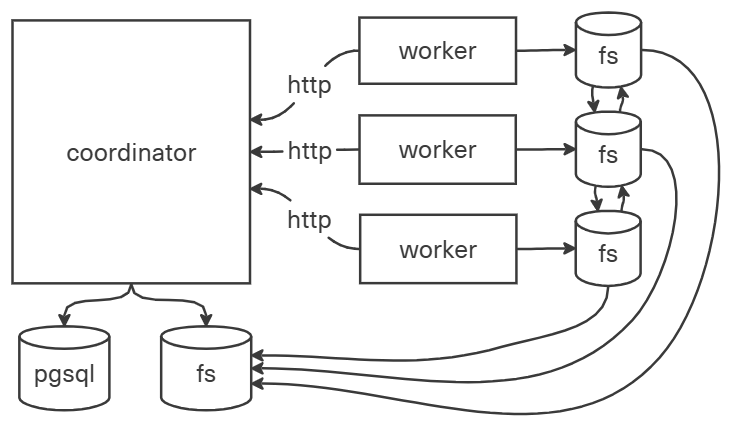
\includegraphics{images/exesh-architecture.png}
}
\caption{
\label{exesh-architecture}
     Архитектура компонентов внутри приложения Exesh.}
\end{center}
\end{figure}

Кластер представляет собой объединение одного coordinator и набора workers.
Горизонтальное масштабирование может быть достигнуто при помощи увеличения количества workers в кластере либо количества кластеров.
После запуска каждый worker регистрируется у заранее определённого coordinator,
а затем с некоторым интервалом выполняет запросы heartbeat для получения новых и передачи результатов выполненных команд.

Каждый coordinator и worker взаимодействует с локальным хранилищем при помощи библиотеки filestorage.
Результатом выполнения каждой команды является артефакт, который сохраняется в локальное хранилище.
Артефакты передаются между компонентами системы также при помощи библиотеки filestorage,
которая реализует передачу ресурсов в формате tar-stream с использованием сжатия.

\subsection{Компонент мониторинга работы системы}

Компонент Dashboard представляет собой приложение на Python с использованием библиотеки Django
и предназначен для визуализации работы Exesh в режиме реального времени.

Изначально для мониторинга планировалось использовать Grafana для сбора метрик и отрисовки дашбордов,
однако для графиков требуется высокая детализация временных событий,
так как за маленький промежуток времени может произойти много изменений.
Поэтому было принято решение реализовать своё приложение,
которое получает из БД все необходимые данные и формирует изображения с графиками.

\subsection{Взаимодействие компонентов}

Frontend и Duely имеют постоянное web-socket соединение,
с помощью которого достигается быстрота обновления интерфейса после каких-либо событий.
Все бэкенд-компоненты предоставляют REST API для взаимодействия с ними.
Для устранения циклических зависимостей и жёсткой связанности между компонентами,
а также для реализации асинхронного взаимодействия внутри некоторых процессов используется брокер обмена сообщениями.
В данном случае выбрана Kafka,
так как предоставляет средства горизонтального масштабирования и обеспечивает отказоустойчивую доставку сообщений.

\subsubsection*{Тестирование решений}

Тестирование решения инициируется пользователем на Frontend и задействует все основные компоненты системы.
Процесс представлен на рисунке \ref{testing-pipeline}.

\begin{figure}[ht]
\begin{center}
\scalebox{0.5}{
   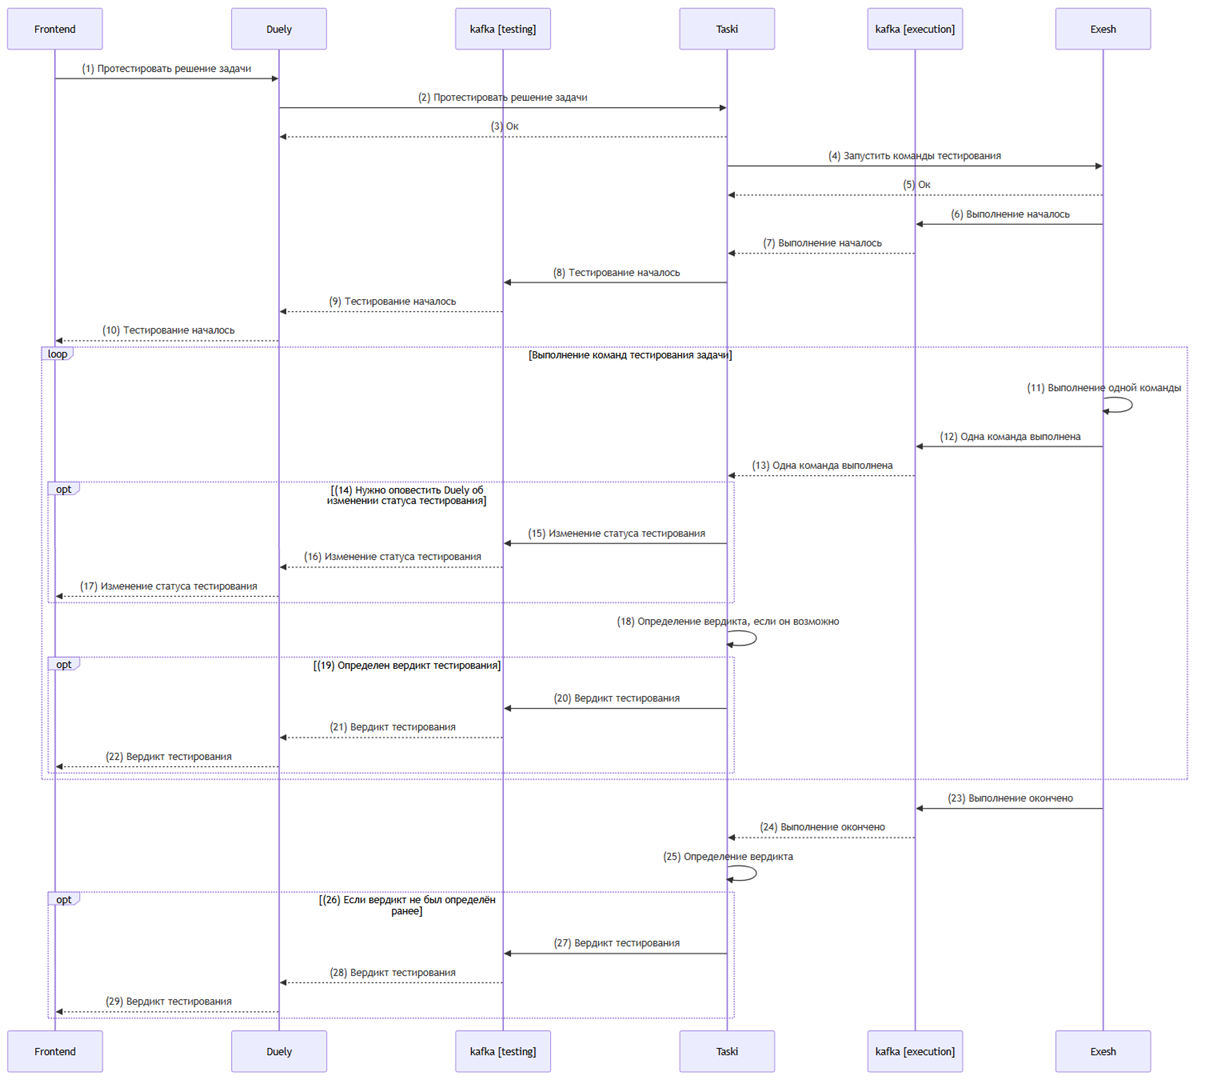
\includegraphics{images/testing-pipeline.png}
}
\caption{
\label{testing-pipeline}
     Процесс тестирования решения.}
\end{center}
\end{figure}

Frontend имеет web-socket соединение с Duely через nginx и отправляет обычный http запрос на тестирование решения задачи (1),
а далее ожидает сообщения с изменением статуса тестирования в web-socket соединение.
Duely выполняет http запрос в Taski на тестирование решения задачи (2)
и при успешном ответе (3) далее ожидает сообщения с изменением статуса тестирования в kafka из топика testing.
Taski делает http запрос в Exesh на запуск команд тестирования решения задачи (4)
и при успешном ответе (5) далее ожидает сообщения с результатами выполнения команд в kafka из топика execution.
Exesh при запуске команд отправляет сообщение о начале выполнения команд в kafka в топик execution (6).
Taski при получении сообщения о начале выполнения команд (7) отправляет сообщение о начале тестирования в kafka в топик testing (8).
Duely при получении сообщения о начале тестирования (9) отправляет сообщение
о начале тестирования в web-socket соединение с Frontend (10).
Exesh при выполнении каждой команды (11) отправляет событие о выполнении команды в kafka в топик execution (12).
Taski при получении сообщения о выполнении команды (13) отправляет сообщение
об изменении статуса тестирования в kafka в топик testing (15), если нужно оповестить Duely об этом (14).
Duely при получении сообщения об изменении статуса тестирования отправляет сообщение
об изменении статуса тестирования в web-socket соединение с Frontend (16).
Taski после получения каждого сообщения о выполнении команд (13) определяет вердикт тестирования (18),
если его можно определить (19), и отправляет его в kafka в топик testing (20).
Exesh при окончании выполнения команд отправляет сообщение о завершении выполнения команд в kafka в топик execution (23).
Taski при получении сообщения об окончании выполнения команд (24) определяет вердикт тестирования (25),
если он не был определен ранее (26), и отправляет его в kafka в топик testing (27).
Duely при получении сообщения с вердиктом (21, 28) тестирования отправляет его в web-socket соединение с Frontend (22, 29).

\subsubsection*{Выполнение кода на входных данных}

При написании кода пользователем в редакторе кода на странице платформы возникает потребность
запуска этого кода на произвольных входных данных с целью получить результат работы кода и отловить ошибки.
Выполнение кода не задействует компонент Taski, так как для него не требуются никакие данные о задаче.
Процесс представлен на рисунке \ref{run-code-pipeline}.

\begin{figure}[ht]
\begin{center}
\scalebox{0.8}{
   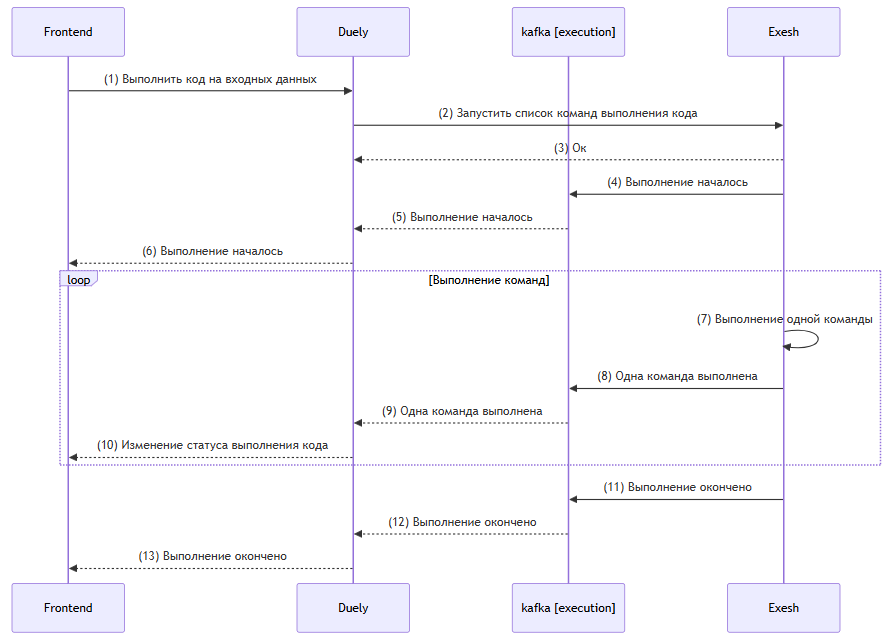
\includegraphics{images/run-code-pipeline.png}
}
\caption{
\label{run-code-pipeline}
     Процесс запуска кода.}
\end{center}
\end{figure}

Frontend имеет web-socket соединение с Duely через nginx и отправляет обычный http запрос на запуск кода (1),
а далее ожидает сообщения с изменением статуса выполнения кода в web-socket соединение.
Duely отправляет http запрос в Exesh на запуск команд выполнения кода (2)
и при успешном ответе (3) далее ожидает сообщения с результатами выполнения команд в kafka из топика execution.
Exesh при запуске команд отправляет сообщение о начале выполнения команд в kafka в топик execution (4).
Duely при получении сообщения о начале выполнения команд (5) отправляет сообщение
о начале выполнения кода в web-socket соединение с Frontend (6).
Exesh при выполнении каждой команды (7) отправляет событие о выполнении команды в kafka в топик execution (8).
Duely при получении сообщения о выполнении команды (9) отправляет сообщение
об изменении статуса выполнения кода в web-socket соединение с Frontend (10).
Exesh при окончании выполнения команд отправляет сообщение о завершении выполнения команд в kafka в топик execution (11).
Duely при получении сообщения об окончании выполнения команд (12)
отправляет в web-socket соединение с Frontend сообщение об окончании выполнения кода (13).

\subsubsection*{Выполнение команд тестирования решений}

При запросе на запуск команд тестирования решения Coordinator сначала сохраняет список команд в БД,
а затем в фоновом процессе вычитывает из БД появившиеся списки команд и начинает их выполнение.
Процесс выполнения списка команд представлен на рисунке \ref{execution-pipeline}.

\begin{figure}[ht]
\begin{center}
\scalebox{0.7}{
   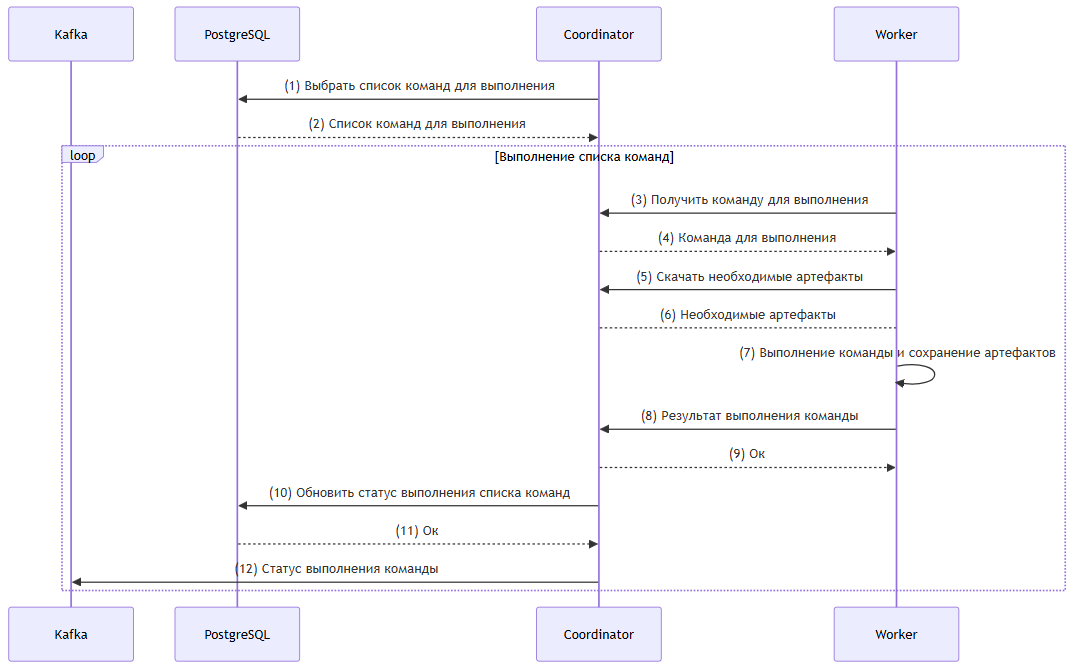
\includegraphics{images/execution-pipeline.png}
}
\caption{
\label{execution-pipeline}
     Процесс выполнения команд тестирования решений.}
\end{center}
\end{figure}

Coordinator выбирает очередной список команд для выполнения из PostgreSQL (1, 2).
Worker с заданным интервалом делает heartbeat-запрос (3) и получает команду для выполнения (4).
Для выполнения команды Worker скачивает необходимые артефакты (5, 6).
После выполнения команды Worker выполняет сохранение артефактов (7).
С результатом выполнения команды (8) Worker идёт в Coordinator (9).
Coordinator обновляет статус выполнения списка команд (10, 11) и отправляет статус выполнения команды в Kafka (12).

\subsubsection*{Анализ подозрительности поведения пользователя}

Для анализа подозрительности поведения Frontend собирает список действий пользователя в интерфейсе.
Analyzer по списку действий пользователя выдаёт степень подозрительности его поведения.
Процесс представлен на рисунке \ref{analyze-pipeline}.

\begin{figure}[ht]
\begin{center}
\scalebox{0.7}{
   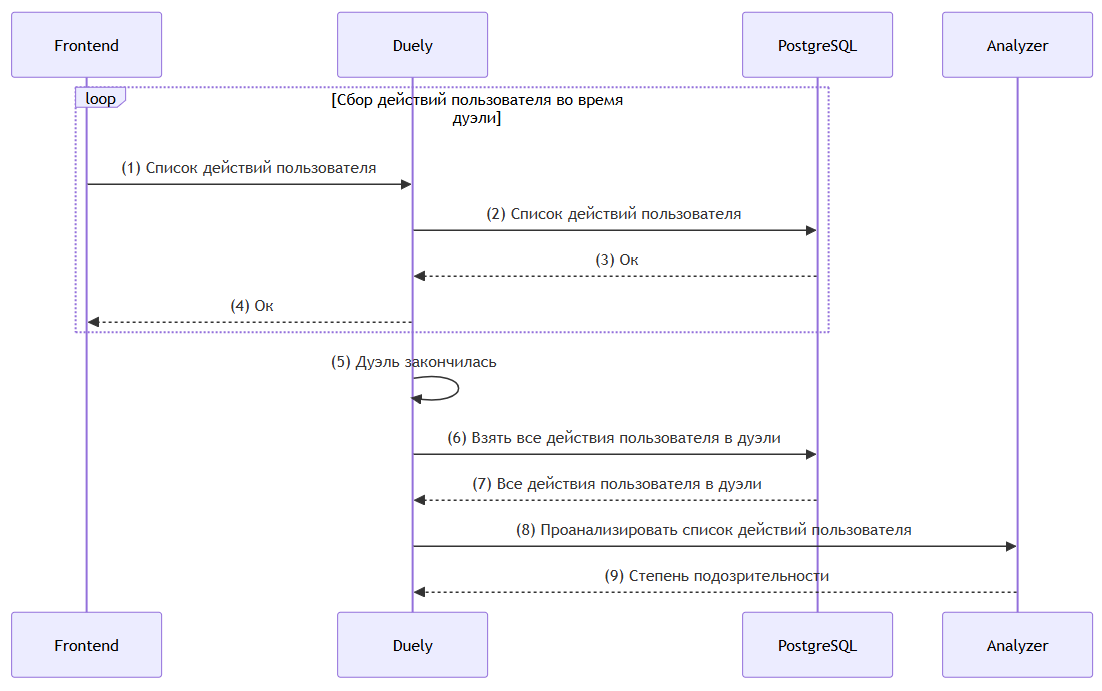
\includegraphics{images/analyze-pipeline.png}
}
\caption{
\label{analyze-pipeline}
     Процесс анализа поведения пользователя.}
\end{center}
\end{figure}

Во время дуэли Frontend собирает список действий пользователя и с заданным интервалом передаёт его в Duely (1, 4).
Duely сохраняет их в PostgreSQL (2, 3).
После окончания дуэли (5) Duely берёт все сохранённые действия пользователя в дуэли из PostgreSQL (6, 7).
Для анализа списка действий пользователя Duely делает запрос в Analyzer (8) и в ответе получает степень подозрительности (9).
